\documentclass[11pt,a4paper]{article}
\usepackage{amssymb}
\usepackage{amsmath}
\usepackage{graphicx}
\usepackage{amscd}
\usepackage{vmargin}
\usepackage{mathrsfs,color,comment}
\usepackage{multirow}
\usepackage{cases}
\usepackage{xfrac}
\usepackage{amsthm}
\usepackage{parskip}
\usepackage{mathtools}
\usepackage{xparse}
\usepackage{algorithm}
\usepackage{algpseudocode}
\usepackage{biblatex}
\usepackage{listings}
\usepackage{matlab-prettifier}
\usepackage{marvosym}
\usepackage{subcaption}
\usepackage{enumerate}

\usepackage{tikz}
\usetikzlibrary {automata,positioning, calc}
%%
%%MARGES
\setmarginsrb{1.2cm}{1.3cm}{1.2cm}{1.3cm}{0cm}{0cm}{0cm}{0cm}
\newtheorem{lemma}{Lemma}
\newtheorem*{lemmas}{Lemmas}

%%%%%%%%%%%%%%%%%%%%%%%%%%%%%%%%%%%%
%%%%%%%%%%%%%%%%%%%%%%%%%%%%%%%%%%%%

%% NOUVELLES COMMANDES

\newcommand\norm[1]{\left\lVert#1\right\rVert}
\newcommand\sym{\mathcal{S}}

\newcommand{\scrP}{\mathscr{P}}
\newcommand{\tr}{\mathrm{tr}}

%%\BB
\newcommand{\QQ}{\mathbb{Q}}
\newcommand{\WW}{\mathbb{W}}
\newcommand{\EE}{\mathbb{E}}
\newcommand{\RR}{\mathbb{R}}
\newcommand{\TT}{\mathbb{T}}
\newcommand{\YY}{\mathbb{Y}}
\newcommand{\UU}{\mathbb{U}}
\newcommand{\II}{\mathbf{1}}
\newcommand{\OO}{\mathbb{O}}
\newcommand{\PP}{\mathbb{P}}
\renewcommand{\AA}{\mathbb{A}}
\renewcommand{\SS}{\mathbb{S}}
\newcommand{\DD}{\mathbb{D}}
\newcommand{\FF}{\mathbb{F}}
\newcommand{\GG}{\mathbb{G}}
\newcommand{\HH}{\mathbb{H}}
\newcommand{\JJ}{\mathbb{J}}
\newcommand{\KK}{\mathbb{K}}
\newcommand{\LL}{\mathbb{L}}
\newcommand{\ZZ}{\mathbb{Z}}
\newcommand{\XX}{\mathbb{X}}
\newcommand{\CC}{\mathbb{C}}
\newcommand{\VV}{\mathbb{V}}
\newcommand{\BB}{\mathbb{B}}
\newcommand{\NN}{\mathbb{N}}
\newcommand{\MM}{\mathbb{M}}


%%\CAL
\newcommand{\A}{\mathcal{A}}
\newcommand{\B}{\mathcal{B}}
\newcommand{\C}{\mathcal{C}}
\newcommand{\D}{\mathcal{D}}
\newcommand{\E}{\mathcal{E}}
\newcommand{\F}{\mathcal{F}}
\newcommand{\G}{\mathcal{G}}
\renewcommand{\H}{\mathcal{H}}
\newcommand{\I}{\mathcal{I}}
\newcommand{\J}{\mathcal{J}}
\newcommand{\K}{\mathcal{K}}
\renewcommand{\L}{\mathcal{L}}
\newcommand{\M}{\mathcal{M}}
\newcommand{\N}{\mathcal{N}}
\renewcommand{\O}{\mathcal{O}}
\renewcommand{\P}{\mathcal{P}}
\newcommand{\Q}{\mathcal{Q}}
\newcommand{\R}{\mathcal{R}}
\renewcommand{\S}{\mathcal{S}}
\newcommand{\T}{\mathcal{T}}
\newcommand{\U}{\mathcal{U}}
\newcommand{\V}{\mathcal{V}}
\newcommand{\W}{\mathcal{W}}
\newcommand{\X}{\mathcal{X}}
\newcommand{\Y}{\mathcal{Y}}
\newcommand{\Z}{\mathcal{Z}}

%%\scr
\newcommand{\Ac}{\mathscr{A}}
\newcommand{\Bc}{\mathscr{B}}
\newcommand{\Cc}{\mathscr{C}}
\newcommand{\Dc}{\mathscr{D}}
\newcommand{\Ec}{\mathscr{E}}
\newcommand{\Fc}{\mathscr{F}}
\newcommand{\Gc}{\mathscr{G}}
\newcommand{\Hc}{\mathscr{H}}
\newcommand{\Ic}{\mathscr{I}}
\newcommand{\Jc}{\mathscr{J}}
\newcommand{\Kc}{\mathscr{K}}
\newcommand{\Lc}{\mathscr{L}}
\newcommand{\Mc}{\mathscr{M}}
\newcommand{\Nc}{\mathscr{N}}
\newcommand{\Oc}{\mathscr{O}}
\newcommand{\Pc}{\mathscr{P}}
\newcommand{\Qc}{\mathscr{Q}}
\newcommand{\Rc}{\mathscr{R}}
\newcommand{\Sc}{\mathscr{S}}
\newcommand{\Tc}{\mathscr{T}}
\newcommand{\Uc}{\mathscr{U}}
\newcommand{\Vc}{\mathscr{V}}
\newcommand{\Wc}{\mathscr{W}}
\newcommand{\Xc}{\mathscr{X}}
\newcommand{\Yc}{\mathscr{Y}}
\newcommand{\Zc}{\mathscr{Z}}

\usepackage{titlesec}
% Make \section look like normal text
\titleformat{\section}[runin]   % "runin" = same line, no big break
  {\normalfont\normalsize\bfseries} % style: normal text size + bold
  {}                             % no number
  {0pt}                          % no space before text
  {}                             % code before the title

\titlespacing*{\section}
  {0pt}{1em}{0.5em} % {left}{before}{after}
\titleformat{\subsection}[runin]{\bfseries}{}{}{}[]
\titleformat{\subsubsection}[runin]{\bfseries}{}{}{}[]

%%EXERCICE
\newcounter{exo}
\newcounter{parti}

\def\exercice%
{\stepcounter{exo}\noindent{\bf Exercise \arabic{parti}.\arabic{exo}.} \ }%
{\vspace{0,3cm}}

\def\partie%
{\stepcounter{parti} \noindent {\bf \arabic{parti}.} --- }%
{\vspace{0,3cm}}

\def\exercices%
{\noindent{\bf Exercises.} \ }%
{\vspace{0,3cm}}


%%%%%%%%%%%%%%%%%%%%%%%
%%%%%%%%%%%%%%%%%%%%%%%

\def\NN{{\mathbb{N}}}
\def\ZZ{{\mathbb{Z}}}
\def\QQ{{\mathbb{Q}}}
\def\RR{{\mathbb{R}}}
\def\CC{{\mathbb{C}}}

\newcommand{\rank}{\mathrm{rank}}
\newcommand{\im}{\mathrm{Im}}

\NewDocumentCommand{\myarrow}{sm}{
  \IfBooleanTF{#1}{
    \xrightarrow{#2}
  }{
    \xrightarrow{\mathmakebox[\minarrow]{#2}}
  }
}
\renewcommand{\arraystretch}{2}


%% DEBUT
\usepackage[utf8]{inputenc}

\pagestyle{empty}

\setlength{\parindent}{0em}
% \renewcommand{\labelitemi}{\scriptsize$\blacksquare$}
\makeatletter
\renewcommand*\env@matrix[1][*\c@MaxMatrixCols c]{%
  \hskip -\arraycolsep
  \let\@ifnextchar\new@ifnextchar
  \array{#1}}
\makeatother
\def\env@matrix{\hskip -\arraycolsep
  \let\@ifnextchar\new@ifnextchar
  \array{*\c@MaxMatrixCols c}}

\makeatletter
% Reinsert missing \algbackskip
\def\algbackskip{\hskip-\ALG@thistlm}
\makeatother
\addbibresource{refs.bib}
\begin{document}

\thispagestyle{empty}
%%ENTETE
\begin{center}
  \textsc{Universit\'e Gustave Eiffel} \hfill  \,\\
  M2 -- Semester 1 -- 2025/2026 \hfill \, \\
\end{center}

\vspace{0.5cm}

\section{Exercise 1.} Describe in detail a Turing machine that decides the language
$$\L=\{w\in \{0,1\}^* \,|\, w \text{ contains equally 0s and 1s}\}.$$

We use the convention that the head points to the symbol right after the start symbol $\triangleright$. We need another symbol $2$ in our alphabet. The idea is that when the string is on the tape, we will traverse it multiple times and at each time, we modify a pair of $0$ and $1$ to $2$ and $2$. A string is in $\L$ if it can be modified to a string of all $2$'s.
\begin{itemize}
  \item At the state $q_\text{init}$, if the tape contains all $2$'s followed by blanks, the original input is accepted. If $0$ is read, the machine goes to the state $q_1$. If $1$ is read, the machine goes to the state $q_2$.
  \item At the state $q_1$, we wait for a $1$, so we loop around when encountering a $0$ or $2$. If a blank is encountered before a $1$ can be read, the string is rejected. If there is a $1$, we move to state $q_3$. Similarly, $q_2$ is the state where we intend to wait for a $0$.
  \item At the state $q_3$, we move to the left until encountering $\triangleright$, by which we move back to $q_\text{init}$ and start reading the next symbol.
\end{itemize}

\begin{figure}[ht]
  \centering
  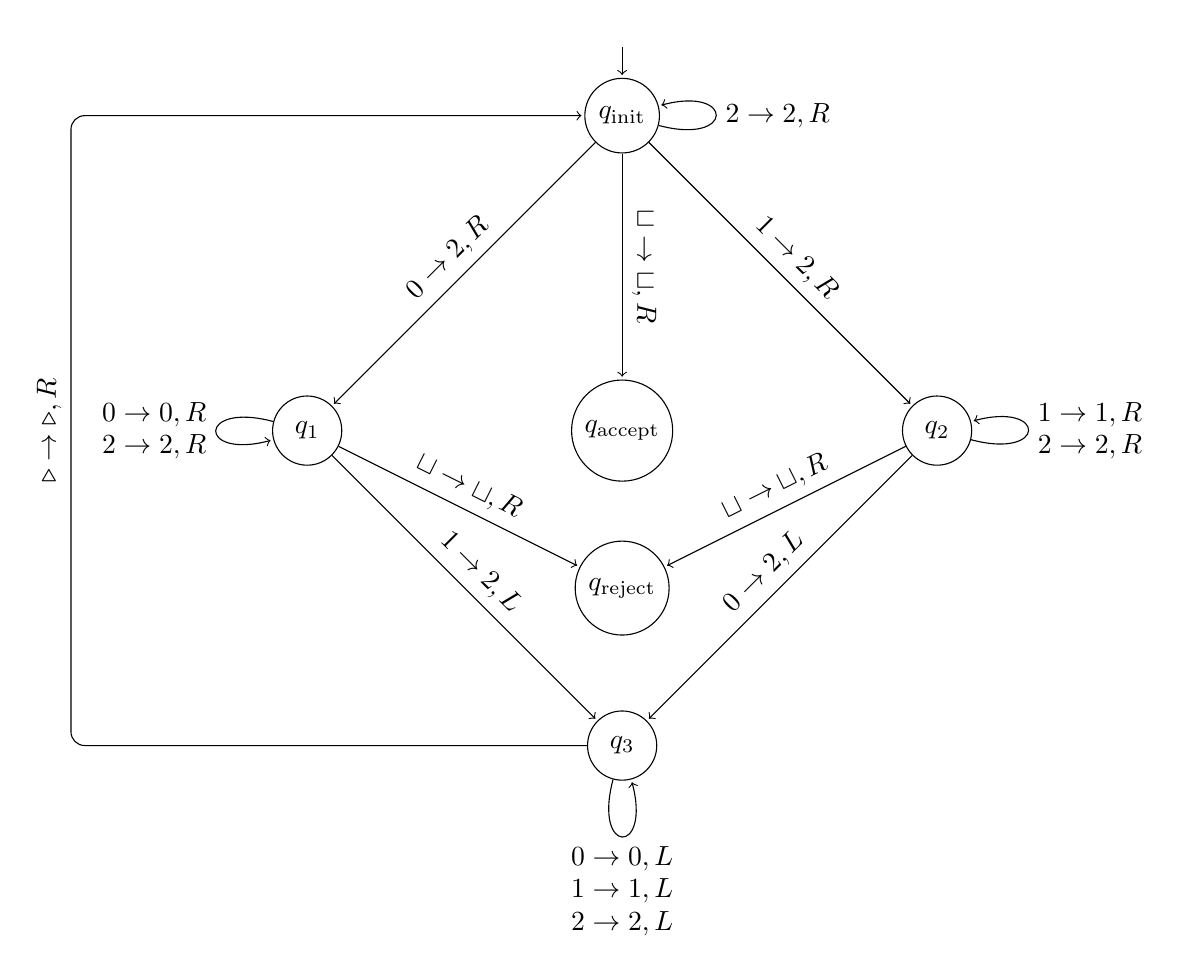
\begin{tikzpicture}[shorten >=1pt,node distance=2cm,on grid,auto]

    \node (init) {};
    \node[state] (q_init) [below=1cm of init] {$q_\text{init}$};
    \node[state] (q1) [below=4cm of q_init, xshift=-4cm] {$q_1$};
    \node[state] (q2) [below=4cm of q_init, xshift=4cm] {$q_2$};
    \node[state] (q_accept) [below=4cm of q_init] {$q_\text{accept}$};
    \node[state] (q_reject) [below=2cm of q_accept] {$q_\text{reject}$};
    \node[state] (q3) [below=4cm of q_accept] {$q_3$};

    \path[->]
    (init) edge node {} (q_init)
    (q_init) edge node[sloped, above] {$0 \to 2, R$} (q1)
    (q_init) edge node[sloped, above] {$1 \to 2, R$} (q2)
    (q_init) edge node[sloped, above] {$\sqcup \to \sqcup, R$} (q_accept)

    (q_init) edge[loop, out=-15, in=15, distance=1cm] node[anchor=west] {$2\to 2, R$} (q_init)

    (q1) edge[loop, out=165, in=195, distance=1cm] node[anchor=east] {\shortstack{$0 \to 0, R$ \\ $2 \to 2, R$}}
    (q1)
    (q1) edge node[sloped, above] {$\sqcup \to \sqcup, R$} (q_reject)
    (q1) edge node[sloped, above] {$1 \to 2, L$} (q3)

    (q2) edge[loop, out=-15, in=15, distance=1cm] node[anchor=west] {\shortstack{$1 \to 1, R$ \\ $2 \to 2, R$}}
    (q2)
    (q2) edge node[sloped, above] {$\sqcup \to \sqcup, R$} (q_reject)
    (q2) edge node[sloped, above] {$0 \to 2, L$} (q3)


    (q3) edge[loop, out=-105, in=-75, distance=1cm] node[anchor=north] {$\shortstack{$0 \to 0, L$ \\ $1 \to 1, L$ \\ $2 \to 2, L$}$} (q3);

    \draw[->, rounded corners=5pt]
    (q3) -- ($(q3)+(-7cm,0)$)
    -- node[sloped, above] {$\triangleright\to\triangleright, R$} ($(q_init)+(-7cm,0)$)
    -- (q_init);

    % (q3) edge[out=180, in=180, distance=9cm] node[sloped, below] {$\triangleright\to\triangleright, R$} (q_init)
    ;
  \end{tikzpicture}
\end{figure}

\section{Exercise 2.} Describe a TM that decides the language $\L=\{w\#w \,|\, w\in\{0,1\}^*\}$.

The idea is similar to Exercise 1. The difference is that if $0$ is encountered, we \textit{wait for another $0$ only after $\#$}. The case of encountering $1$ is the same.

\begin{figure}[ht]
  \centering
  \begin{tikzpicture}[shorten >=1pt,node distance=2cm,on grid,auto]

    \node (init) {};
    \node[state] (q_init) [below=1cm of init] {$q_\text{init}$};
    \node[state] (q1) [below=4cm of q_init, xshift=-4cm] {$q_1$};
    \node[state] (q1') [below=4cm of q1] {$q_1'$};
    \node[state] (q2) [below=4cm of q_init, xshift=4cm] {$q_2$};
    \node[state] (q2') [below=4cm of q2] {$q_2'$};
    \node[state] (q_accept) [below=4cm of q_init] {$q_\text{accept}$};
    \node[state] (q_reject) [below=4cm of q_accept] {$q_\text{reject}$};
    \node[state] (q3) [below=8cm of q_accept] {$q_3$};

    \path[->]
    (init) edge node {} (q_init)
    (q_init) edge node[sloped, above] {$0 \to 2, R$} (q1)
    (q_init) edge node[sloped, above] {$1 \to 2, R$} (q2)
    (q_init) edge node[sloped, above] {$\sqcup \to \sqcup, R$} (q_accept)

    (q_init) edge[loop, out=-15, in=15, distance=1cm] node[anchor=west] {$2\to 2, R$} (q_init)

    (q1) edge[loop, out=165, in=195, distance=1cm] node[anchor=east] {\shortstack{$0 \to 0, R$ \\ $1 \to 1, R$ \\ $2 \to 2, R$}}
    (q1)

    (q1) edge node[sloped, above] {$\# \to \#, R$} (q1')

    (q1') edge[loop, out=165, in=195, distance=1cm] node[anchor=east] {$2 \to 2, R$}
    (q1')
    (q1') edge node[sloped, above] {$1 \to 1, R$} (q_reject)
    (q1') edge node[sloped, above] {$0 \to 2, L$} (q3)

    (q2) edge[loop, out=-15, in=15, distance=1cm] node[anchor=west] {\shortstack{$0 \to 0, R$ \\ $1 \to 1, R$ \\ $2 \to 2, R$}}
    (q2)

    (q2) edge node[sloped, above] {$\# \to \#, R$} (q2')

    (q2') edge[loop, out=-15, in=15, distance=1cm] node[anchor=west] {$2 \to 2, R$}
    (q2')
    (q2') edge node[sloped, above] {$0 \to 0, R$} (q_reject)
    (q2') edge node[sloped, above] {$1 \to 2, L$} (q3)


    (q3) edge[loop, out=-105, in=-75, distance=1cm] node[anchor=north] {$\shortstack{$0 \to 0, L$ \\ $1 \to 1, L$ \\ $2 \to 2, L$ \\  $\# \to \#, L$}$} (q3)
    ;

    \draw[->, rounded corners=5pt]
    (q3) -- ($(q3)+(-7cm,0)$)
    -- node[sloped, above] {$\triangleright\to\triangleright, R$} ($(q_init)+(-7cm,0)$)
    -- (q_init);
  \end{tikzpicture}
\end{figure}

\section{Exercise 5.} Let $\L(M)$ be the language recognized by the TM $M$ i.e. the set of inputs $w\in\{0,1\}^*$ such that $M$ halts with output $1$ (on other inputs it may halt with output 0 or not halt). Consider the problem $E_\text{TM} = \{\langle M\rangle \,|\, M \text{ is a TM and } \L(M)=\varnothing\}$. Show that if $E_\text{TM}$ were decidable, then the halting problem would also be decidable. Conclude that $E_\text{TM}$ is undecidable.

For any encoding $\langle M,w\rangle$ of a TM and an input, construct a TM $M'$ such that
\begin{itemize}
  \item If $\forall x\in \{0,1\}^*, M'(x) = 1$ or $\L(M') = \{0,1\}^*$, then $M$ halts on $w$;
  \item If $\forall x\in \{0,1\}^*, M'(x)$ does not halt or $\L(M') = \varnothing$, then $M$ does not halt on $w$.
\end{itemize}

If $E_\text{TM}$ were decidable, then there would be a TM $N$ such that
$$N(\langle M'\rangle) = 1 \Leftrightarrow \L(M') = \varnothing \Leftrightarrow \text{ $M$ does not halt on $w$},$$
$$N(\langle M'\rangle) = 0 \Leftrightarrow \L(M') \neq \varnothing \Leftrightarrow \text{$M$ halts on $w$}.$$
So it would be possible to use $N$ to decide if a TM $M$ halts or not, or the halting problem would be decidable. But in fact, it is not. Thus, $E_\text{TM}$ is undecidable.

\printbibliography

\end{document}